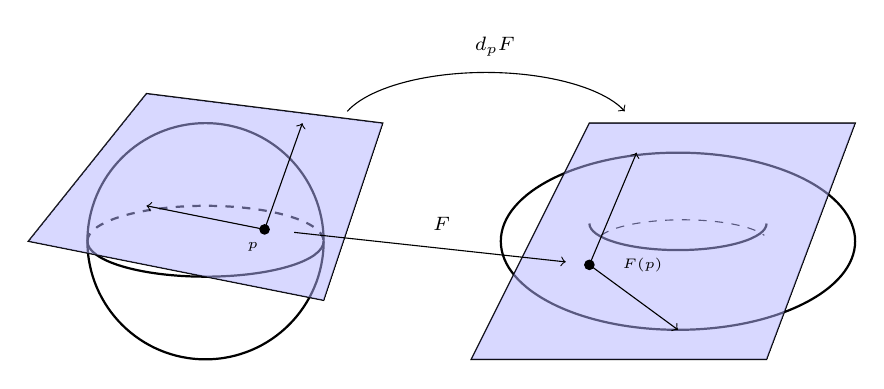
\begin{tikzpicture}[scale=1.5]
	% Esfera
	\draw [thick] (-1,0) arc (0:180:1 and -0.3);
	\draw [thick, dashed] (-3,0) arc (180:0:1 and 0.3);
	\draw [thick] (-2,0) circle (1);

	% Espacio Tangente a Esfera
	\draw [line width=0.5] (-3.5,0) -- (-2.5,1.25) -- (-0.5,1) -- (-1,-0.5) -- cycle;
	\draw [fill=blue!30!white,opacity=0.5, line width=0] (-3.5,0) -- (-2.5,1.25) -- (-0.5,1) -- (-1,-0.5) -- cycle;

	% Punto $a$
	\filldraw (-1.5,0.1) circle (0.04);
	\node at (-1.60,-0.05) {\tiny $p$};

	% Vector en $a$
	\draw [->] (-1.5,0.1) -- (-1.18,1);
	\draw [->] (-1.5,0.1) -- (-2.5,0.3);

	% Toro
	\draw [thick] (2,0) ellipse  (1.5 and 0.75);
	\draw [thick] (1.25,0.15) arc (0:-180:-0.75 and 0.225);
	\draw [dashed] (1.35,0.05) arc (20:160:-0.735 and 0.2);

	% Espacio tangente a Toro
	\draw [line width=0.5] (1.25,1) -- (3.5,1) -- (2.75,-1) -- (0.25,-1) -- cycle;
	\draw [fill=blue!30!white,opacity=0.5, line width=0] (1.25,1) -- (3.5,1) -- (2.75,-1) -- (0.25,-1) -- cycle;

	% Punto $F(a)$
	\filldraw (1.25,-0.2) circle (0.04);
	\node at (1.7,-0.2) {\tiny $F(p)$};

	% Vector en $F(a)$
	\draw[->] (1.25,-0.2) -- (1.65,0.75);
	\draw[->] (1.25,-0.2) -- (2,-0.75);

	% Lineas
	\draw[->] (-1.25,0.075) -- (1.05,-0.175);
	\node at (0,0.15) {\scriptsize $F$};


	\draw[->] (-0.8,1.1) arc (160:20:1.25 and 0.5);
	\node at (0.45,1.65) {\scriptsize $d_{p}F$};
\end{tikzpicture}
